
\documentclass{book}
\usepackage[landscape,a3paper,left=0.5cm,right=1in,top=1in,bottom=1in]{geometry}
\usepackage{amsmath}
\usepackage{xcolor}
\usepackage{tikz}
\usepackage{pgfplots}
\usepackage{booktabs}
\usepackage{multirow}
\usepackage{amsmath,amssymb}


\newcommand\id[1]{\textsc{#1}}

\begin{document}



\begin{table}[!ht]\scriptsize
\center

\begin{tabular}{|l|l|l|l|l|l|l|l|l|}\toprule Group of & \multirow{2}{*}{ Type of instances} & &\multicolumn{5}{c|}{\% of solved instances among 31} & \% of time out\\
\cmidrule(lr){3-9}
instances &  & Time (min)  & $\leq 1$ & $\leq 10$ & $\leq 30$ & $\leq 150$ & $\leq 1440$ & $> 1440$ \\
\midrule
 \multirow{15}{*}{\id{Small}} & \multirow{3}{*}{\id{Equiv+Permut}} & \textsc{Algo}   & \bf 100.0\% & \bf 100.0\% & \bf 100.0\% & \bf 100.0\% & \bf 100.0\% &  \bf 0.0\% \\
& & \textsc{QuadraMod} + coinbc   & \bf 100.0\% & \bf 100.0\% & \bf 100.0\% & \bf 100.0\% & \bf 100.0\% &  \bf 0.0\% \\
& & \textsc{QuadraMod} + cplex   & 18.18\% & 45.45\% & 72.73\% & 90.91\% & \bf 100.0\% &  \bf 0.0\% \\
\cmidrule(lr){2-9}
 & \multirow{3}{*}{\id{Non-Equiv+Permut}} & \textsc{Algo}   & \bf 100.0\% & \bf 100.0\% & \bf 100.0\% & \bf 100.0\% & \bf 100.0\% &  \bf 0.0\% \\
& & \textsc{PermutMod} + gecode   & 50.0\% & 95.45\% & \bf 100.0\% & \bf 100.0\% & \bf 100.0\% &  \bf 0.0\% \\
& & \textsc{PermutMod} + scip   & 0.0\% & 40.0\% & 60.0\% & \bf 100.0\% & \bf 100.0\% &  \bf 0.0\% \\
\cmidrule(lr){2-9}
 & \multirow{3}{*}{\id{Equiv+Permut+Scaling}} & \textsc{AlgoScale}   & 0\% & 0\% & 0\% & 0\% & 0\% & 100\% \\
& & \textsc{AlgoEnhance2}   & 46.67\% & 80.0\% & \bf 100.0\% & \bf 100.0\% & \bf 100.0\% &  \bf 0.0\% \\
& & \textsc{AlgoEnhance}   & 33.33\% & 33.33\% & 33.33\% & 33.33\% & \bf 100.0\% &  \bf 0.0\% \\
& & \textsc{PermutMod} + gecode   & 57.89\% & \bf 100.0\% & \bf 100.0\% & \bf 100.0\% & \bf 100.0\% &  \bf 0.0\% \\
& & \textsc{QuadraMod} + chuffed   & \bf 66.67\% & 83.33\% & \bf 100.0\% & \bf 100.0\% & \bf 100.0\% &  \bf 0.0\% \\
\cmidrule(lr){2-9}
 & \multirow{3}{*}{\id{Non-Equiv+Permut+Scaling}}& \textsc{AlgoScale}   & 0\% & 0\% & 0\% & 0\% & 0\% & 100\% \\
& & \textsc{AlgoEnhance2}   & 62.5\% & 68.75\% & 68.75\% & 87.5\% & \bf 100.0\% &  \bf 0.0\% \\
& & \textsc{AlgoEnhance}   & 64.29\% & 78.57\% & 78.57\% & 92.86\% & \bf 100.0\% &  \bf 0.0\% \\
& & \textsc{PermutMod} + cp-sat   & \bf 66.67\% & \bf 100.0\% & \bf 100.0\% & \bf 100.0\% & \bf 100.0\% &  \bf 0.0\% \\
\bottomrule\end{tabular}

\end{table}


\begin{table}[!ht]\scriptsize
\center

\begin{tabular}{|l|l|l|l|l|l|l|l|l|}\toprule Group of & \multirow{2}{*}{ Type of instances} & &\multicolumn{5}{c|}{\% of solved instances among 31} & \% of time out\\
\cmidrule(lr){3-9}
instances &  & Time (min)  & $\leq 1$ & $\leq 10$ & $\leq 30$ & $\leq 150$ & $\leq 1440$ & $> 1440$ \\
\midrule
 \multirow{15}{*}{\id{Medium}} & \multirow{3}{*}{\id{Equiv+Permut}} & \textsc{Algo}   & \bf 80.0\% & \bf 100.0\% & \bf 100.0\% & \bf 100.0\% & \bf 100.0\% &  \bf 0.0\% \\
& & \textsc{TheoMod} + gecode   & 0.0\% & 0.0\% & 0.0\% & \bf 100.0\% & \bf 100.0\% &  \bf 0.0\% \\
\cmidrule(lr){2-9}
 & \multirow{3}{*}{\id{Non-Equiv+Permut}} & \textsc{Algo}   & \bf 100.0\% & \bf 100.0\% & \bf 100.0\% & \bf 100.0\% & \bf 100.0\% &  \bf 0.0\% \\
& &\textsc{PermutMod} + chuffed   & 0.0\% & 0.0\% & 0.0\% & 66.67\% & \bf 100.0\% &  \bf 0.0\% \\
& & \textsc{TheoMod} + gecode   & 0.0\% & 0.0\% & 60.0\% & \bf 100.0\% & \bf 100.0\% &  \bf 0.0\% \\
\cmidrule(lr){2-9}
 & \multirow{3}{*}{\id{Equiv+Permut+Scaling}} & \textsc{AlgoScale}   & 0\% & 0\% & 0\% & 0\% & 0\% & 100\% \\
& & \textsc{AlgoEnhance2}   & \bf 0.0\% & \bf 0.0\% & \bf 100.0\% & \bf 100.0\% & \bf 100.0\% &  \bf 0.0\% \\
\cmidrule(lr){2-9}
 & \multirow{3}{*}{\id{Non-Equiv+Permut+Scaling}}& \textsc{AlgoScale}   & 0\% & 0\% & 0\% & 0\% & 0\% & 100\% \\
& & \textsc{AlgoEnhance2}   & \bf 66.67\% & \bf 100.0\% & \bf 100.0\% & \bf 100.0\% & \bf 100.0\% &  \bf 0.0\% \\
& & \textsc{AlgoEnhance}   & \bf 66.67\% & 66.67\% & \bf 100.0\% & \bf 100.0\% & \bf 100.0\% &  \bf 0.0\% \\
\bottomrule\end{tabular}

\end{table}


\begin{figure}
\begin{tabular}{ll}\multicolumn{2}{c}{Small instances}\\
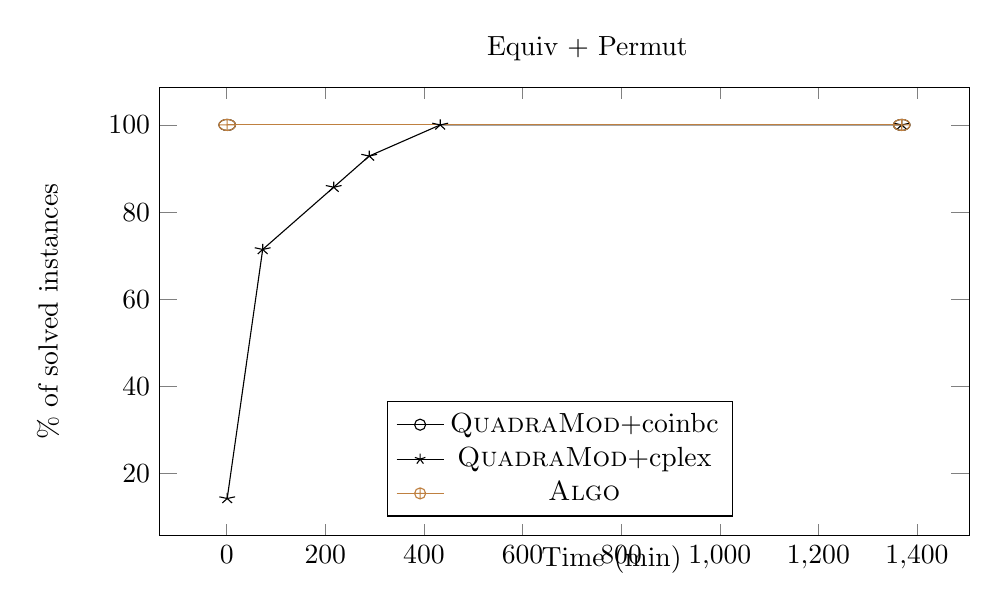
\begin{tikzpicture}
\begin{axis}[scaled ticks=false, xscale=1.5,legend columns = 1, legend style={at={(0.5,0.3)}},
title style={at={(0.38,1)}}, title={Equiv + Permut},xlabel style={at={(0.4,0.0)}},xlabel=Time (min),ylabel=\% of solved instances]
\addplot[color=black,mark=o] coordinates {(1,100.0)
(1369,100.0)
};
\addplot[color=black,mark=star] coordinates {(1,14.29)
(73,71.43)
(217,85.71)
(289,92.86)
(433,100.0)
(1369,100.0)
};
\addplot[color=brown,mark=oplus] coordinates {(1,100.0)
(1369,100.0)
};
%\addplot[color=red,mark=otimes] coordinates {(0,0)
%};
%\addplot[color=teal,mark=triangle] coordinates {(0,0)
%};
\legend{\id{QuadraMod}+coinbc,\id{QuadraMod}+cplex,\id{Algo}}
\end{axis}
\end{tikzpicture}

%\ref{named1} 
& 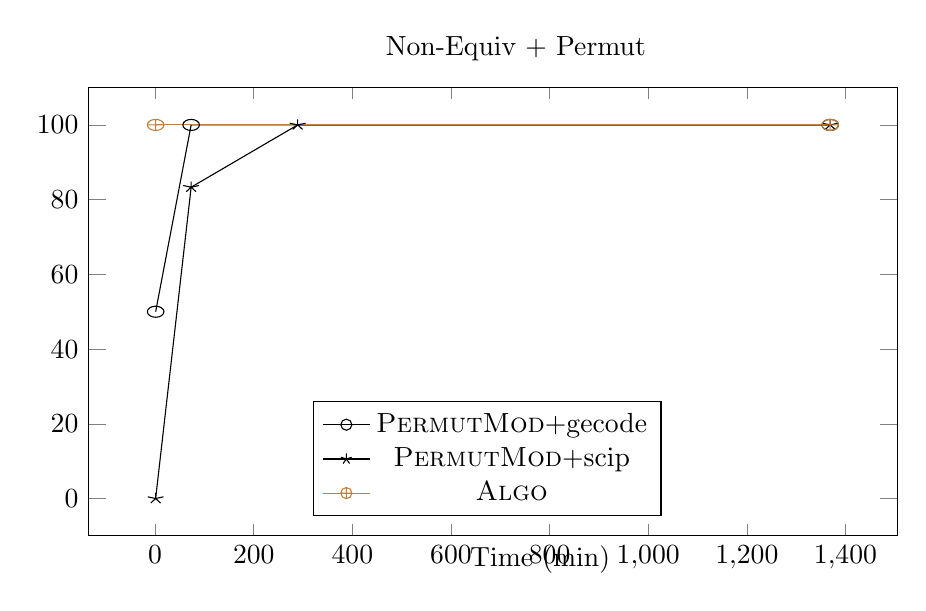
\begin{tikzpicture}
\begin{axis}[scaled ticks=false,xscale=1.5,title style={at={(0.38,1)}},  legend style={at={(0.5,0.3)}},
title={Non-Equiv + Permut},xlabel style={at={(0.4,0.0)}},xlabel=Time (min)]
\addplot[color=black,mark=o] coordinates {(1,50.0)
(73,100.0)
(1369,100.0)
};
\addplot[color=black,mark=star] coordinates {(1,0.0)
(73,83.33)
(289,100.0)
(1369,100.0)
};
\addplot[color=brown,mark=oplus] coordinates {(1,100.0)
(1369,100.0)
};
%\addplot[color=red,mark=otimes] coordinates {(0,0)
%};
%\addplot[color=teal,mark=triangle] coordinates {(0,0)
%};
\legend{\id{PermutMod}+gecode,\id{PermutMod}+scip,\id{Algo}}
\end{axis}
\end{tikzpicture}
 \\
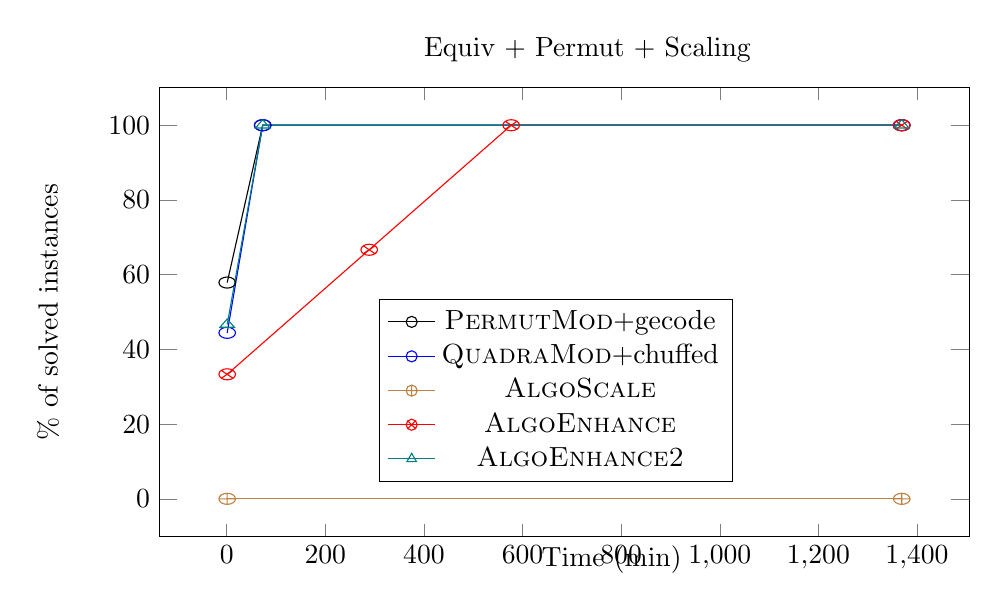
\begin{tikzpicture}
\begin{axis}[scaled ticks=false,xscale=1.5,title style={at={(0.38,1)}},  legend style={at={(0.5,0.53)}},
title={Equiv + Permut + Scaling},xlabel style={at={(0.4,0.0)}},xlabel=Time (min),ylabel=\% of solved instances]
\addplot[color=black,mark=o] coordinates {(1,57.89)
(73,100.0)
(1369,100.0)
};
\addplot[color=blue,mark=o] coordinates {(1,44.44)
(73,100.0)
(1369,100.0)
};
\addplot[color=brown,mark=oplus] coordinates {(1,0)
(1369,0)
};
\addplot[color=red,mark=otimes] coordinates {(1,33.33)
(289,66.67)
(577,100.0)
(1369,100.0)
};
\addplot[color=teal,mark=triangle] coordinates {(1,46.67)
(73,100.0)
(1369,100.0)
};
\legend{\id{PermutMod}+gecode,\id{QuadraMod}+chuffed,\id{AlgoScale},\id{AlgoEnhance},\id{AlgoEnhance2}}
\end{axis}
\end{tikzpicture} &  
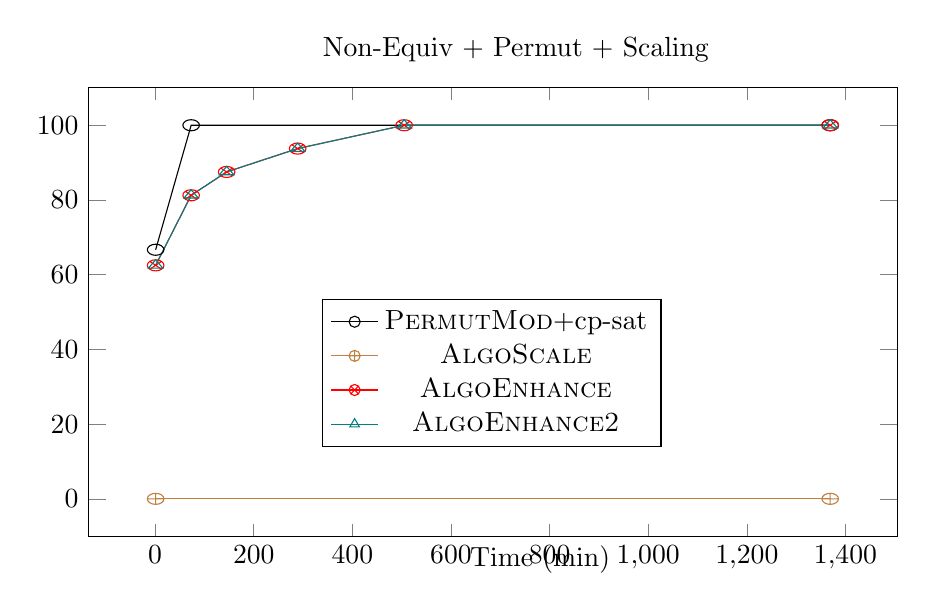
\begin{tikzpicture}
\begin{axis}[scaled ticks=false,xscale=1.5,title style={at={(0.38,1)}},  legend style={at={(0.5,0.53)}},
title={Non-Equiv + Permut + Scaling},xlabel style={at={(0.4,0.0)}},xlabel=Time (min)]
\addplot[color=black,mark=o] coordinates {(1,66.67)
(73,100.0)
(1369,100.0)
};
\addplot[color=brown,mark=oplus] coordinates {(1,0)
(1369,0)
};
\addplot[color=red,mark=otimes] coordinates {(1,62.5)
(73,81.25)
(145,87.5)
(289,93.75)
(505,100.0)
(1369,100.0)
};
\addplot[color=teal,mark=triangle] coordinates {(1,62.5)
(73,81.25)
(145,87.5)
(289,93.75)
(505,100.0)
(1369,100.0)
};
\legend{\id{PermutMod}+cp-sat,\id{AlgoScale},\id{AlgoEnhance},\id{AlgoEnhance2}}
\end{axis}
 \end{tikzpicture}
 \end{tabular}

\end{figure}

%%%%%%%%%%%%%%%%%%%%%%%%%%%%%%%%%%%%%%%%%%%%%%%%%%%%%%%%%%%%%%%%%%%%%%%%%%%%%%%%%%%%%%%%%%%%%
%%%%%%%%%%%%%%%%%%%%%%%%%%%%%%%%%%%%%%%%%%%%%%%%%%%%%%%%%%%%%%%%%%%%%%%%%%%%%%%%%%%%%%%%%%%%%

\begin{figure}
\centering
\begin{tabular}{ll}
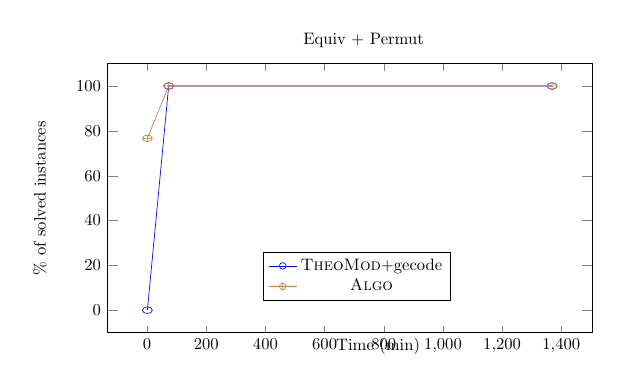
\begin{tikzpicture}[scale = 0.6]
\begin{axis}[scaled ticks=false, xscale=1.5,legend columns = 1, legend style={at={(0.5,0.3)}},
title style={at={(0.38,1)}}, title={Equiv + Permut},xlabel style={at={(0.4,0.0)}},xlabel=Time (min),ylabel=\% of solved instances]
\addplot[color=blue,mark=o] coordinates {(1,0.0)
(73,100.0)
(1369,100.0)
};
\addplot[color=brown,mark=oplus] coordinates {(1,76.67)
(73,100.0)
(1369,100.0)
};
\legend{\id{TheoMod}+gecode,\id{Algo}}
\end{axis}
\end{tikzpicture}

%\ref{named1} 
& 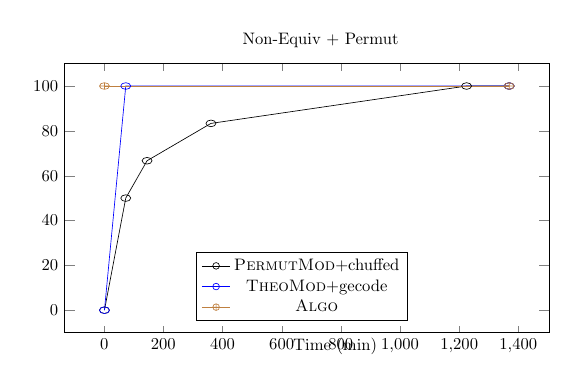
\begin{tikzpicture}[scale = 0.6]
\begin{axis}[scaled ticks=false,xscale=1.5,title style={at={(0.38,1)}},  legend style={at={(0.5,0.3)}},
title={Non-Equiv + Permut},xlabel style={at={(0.4,0.0)}},xlabel=Time (min)]
\addplot[color=black,mark=o] coordinates {(1,0.0)
(73,50.0)
(145,66.67)
(361,83.33)
(1225,100.0)
(1369,100.0)
};
\addplot[color=blue,mark=o] coordinates {(1,0.0)
(73,100.0)
(1369,100.0)
};

\addplot[color=brown,mark=oplus] coordinates {(1,100.0)
(1369,100.0)
};
%\addplot[color=red,mark=otimes] coordinates {(0,0)
%};
%\addplot[color=teal,mark=triangle] coordinates {(0,0)
%};
\legend{\id{PermutMod}+chuffed,\id{TheoMod}+gecode,\id{Algo}}
\end{axis}
\end{tikzpicture}
 \\
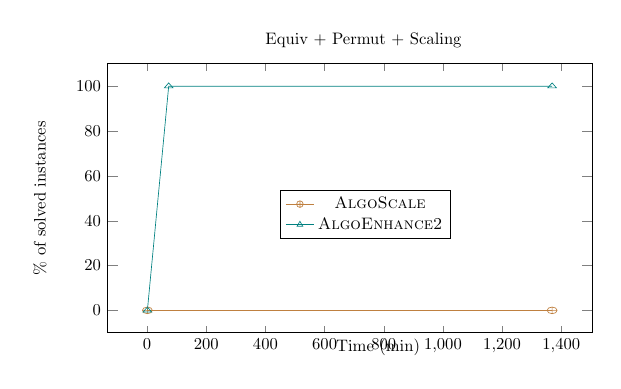
\begin{tikzpicture}[scale = 0.6]
\begin{axis}[scaled ticks=false,xscale=1.5,title style={at={(0.38,1)}},  legend style={at={(0.5,0.53)}},
title={Equiv + Permut + Scaling},xlabel style={at={(0.4,0.0)}},xlabel=Time (min),ylabel=\% of solved instances]
\addplot[color=brown,mark=oplus] coordinates {(1,0)
(1369,0)
};
\addplot[color=teal,mark=triangle] coordinates {(1,0.0)
(73,100.0)
(1369,100.0)
};
\legend{\id{AlgoScale},\id{AlgoEnhance2}}
\end{axis}
\end{tikzpicture} &  
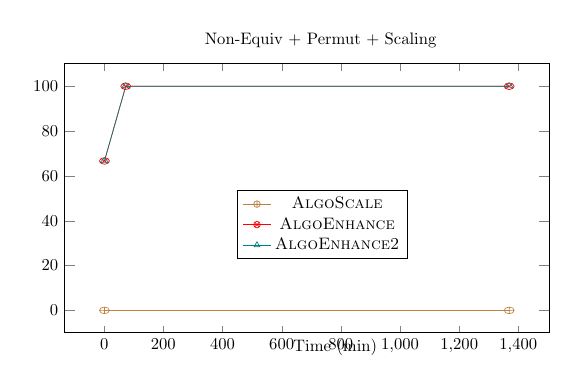
\begin{tikzpicture}[scale = 0.6]
\begin{axis}[scaled ticks=false,xscale=1.5,title style={at={(0.38,1)}},  legend style={at={(0.5,0.53)}},
title={Non-Equiv + Permut + Scaling},xlabel style={at={(0.4,0.0)}},xlabel=Time (min)]
\addplot[color=brown,mark=oplus] coordinates {(1,0)
(1369,0)
};
\addplot[color=red,mark=otimes] coordinates {(1,66.67)
(73,100.0)
(1369,100.0)
};
\addplot[color=teal,mark=triangle] coordinates {(1,66.67)
(73,100.0)
(1369,100.0)
};

\legend{\id{AlgoScale},\id{AlgoEnhance},\id{AlgoEnhance2}}
\end{axis}
 \end{tikzpicture}
 \end{tabular}
\caption{Graphical results for medium instances}
\end{figure}


\end{document}